\documentclass[xcolor=dvipsnames]{beamer}
\usepackage[T1]{fontenc}
\usepackage[utf8]{inputenc}
\usepackage[english,slovak]{babel}

\usepackage{amsmath}
\usepackage{amsthm}
\usetheme{Pittsburgh}
\useoutertheme{shadow}

\usepackage{graphicx}
\usepackage{caption}
\usepackage{subcaption}

\usepackage{tabularx}


\usepackage{listings}
\lstloadlanguages{Ruby}
\lstset{%
basicstyle=\ttfamily\color{black},
commentstyle = \ttfamily\color{red},
keywordstyle=\ttfamily\color{blue},
stringstyle=\color{orange}}



%-------------------------------------------------------------------------------------
\title{\bf Aproximácia funkcie ohodnotení v algoritmoch Q-learning}
\author{Ing. Michal CHOVANEC \\Fakulta riadenia a informatiky}

\date[EURP]{\it Marec 2016}
\begin{document}

\begin{frame}
\titlepage
\end{frame}

%-------------------------------------------------------------------------------------
\begin{frame}{\bf Obsah}

\begin{itemize}
  \item Úvod
    \begin{itemize}
    \item Agentové systémy
    \item Adaptívne a učiace sa systémy
    \end{itemize}
  \item Q-learning algoritmus
  \item Možnosti aproximácie
  \item Výsledky experimentov
\end{itemize}

\end{frame}



%-------------------------------------------------------------------------------------
\begin{frame}{\bf Agentové systémy}

\begin{minipage}{.5\textwidth}

\begin{figure}[!htb]
\centering
\includegraphics[scale=.2]{../pictures/kgb_agent.jpg}
\end{figure}

\begin{figure}[!htb]
\centering
\includegraphics[scale=.4]{../pictures/software_agent.jpg}
\end{figure}

\end{minipage}%
\begin{minipage}{.5\textwidth}

\begin{figure}[!htb]
\centering
\includegraphics[scale=.12]{../pictures/shakey.jpg}
\end{figure}

\begin{figure}[!htb]
\centering
\includegraphics[scale=.25]{../pictures/mars_robot.jpg}
\end{figure}


\end{minipage}


\end{frame}


%-------------------------------------------------------------------------------------
\begin{frame}{\bf Agentové systémy}

Racionálny agent :

\begin{minipage}{.5\textwidth}

  \begin{itemize}
  \item Schopný vnímať prostredie
  \item Robiť rozhodnutia
  \item Pre každú možnú postupnosť vstupov vyberá akciu maximalizujúcu očakavaný výkon
  \end{itemize}

\end{minipage}%
\begin{minipage}{.5\textwidth}

    \begin{figure}[!htb]
    \centering
    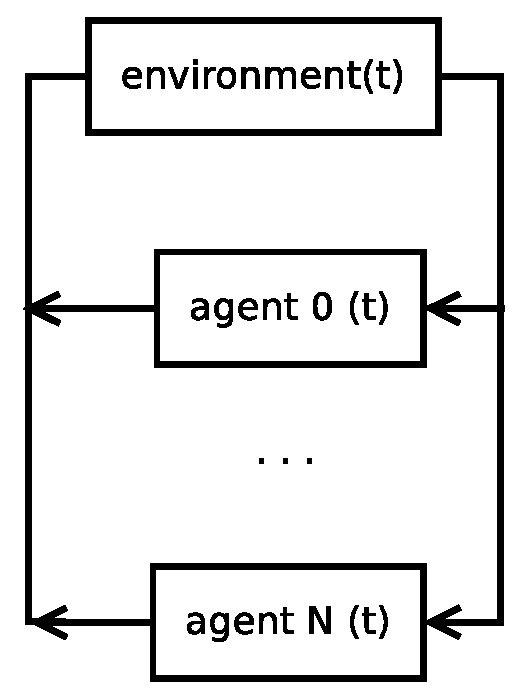
\includegraphics[scale=.3]{../diagrams/multiagent_diagram.eps}
    \caption{Multiagentný systém}
    \label{fig:multiagent_system}
    \end{figure}

\end{minipage}


\end{frame}


%-------------------------------------------------------------------------------------
\begin{frame}{\bf Adaptívne a učiace sa systémy}

\begin{minipage}{.5\textwidth}
  {\bf Adaptívny systém}

  \begin{itemize}
  \item reaktívne správanie
  \item dôraz na čas
  \item nemá pamäť - bez očakávaní
  \item rychlá dynamika
  \end{itemize}

\end{minipage}%
\begin{minipage}{.5\textwidth}
  {\bf Učiaci sa systém}

  \begin{itemize}
  \item konštruktívne správanie
  \item dôraz na priestor
  \item má pamäť - očakávania
  \item pomalá dynamika
  \end{itemize}

\end{minipage}
\end{frame}

%-------------------------------------------------------------------------------------
\begin{frame}{\bf Adaptívne a učiace sa systémy}

\begin{minipage}{.5\textwidth}
  {\bf Adaptívny systém}

  \begin{figure}[!htb]
  \centering
  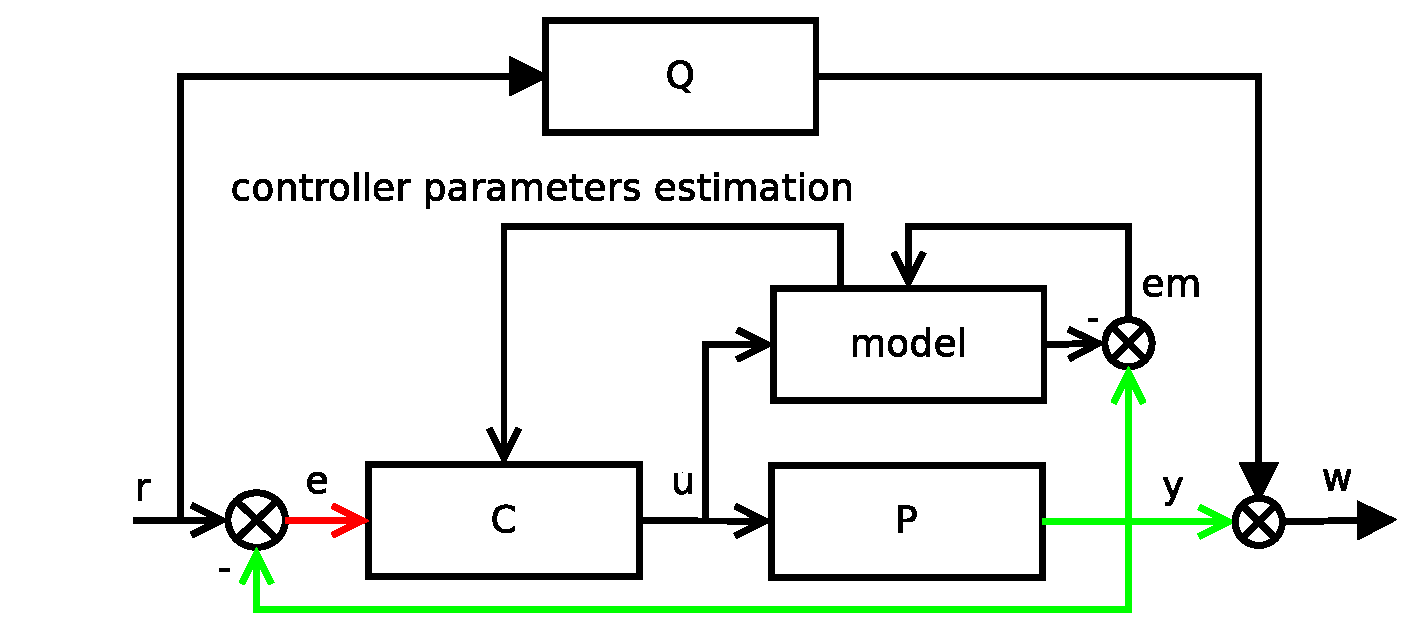
\includegraphics[scale=.22]{../diagrams/adaptive_system.eps}
  \label{fig:adaptive_system}
  \end{figure}

  \begin{figure}[!htb]
  \centering
  \includegraphics[scale=.2]{../pictures/function_f1.png}
  \end{figure}

\end{minipage}%
\begin{minipage}{.5\textwidth}

  {\bf Učiaci sa systém}

  \begin{figure}[!htb]
  \centering
  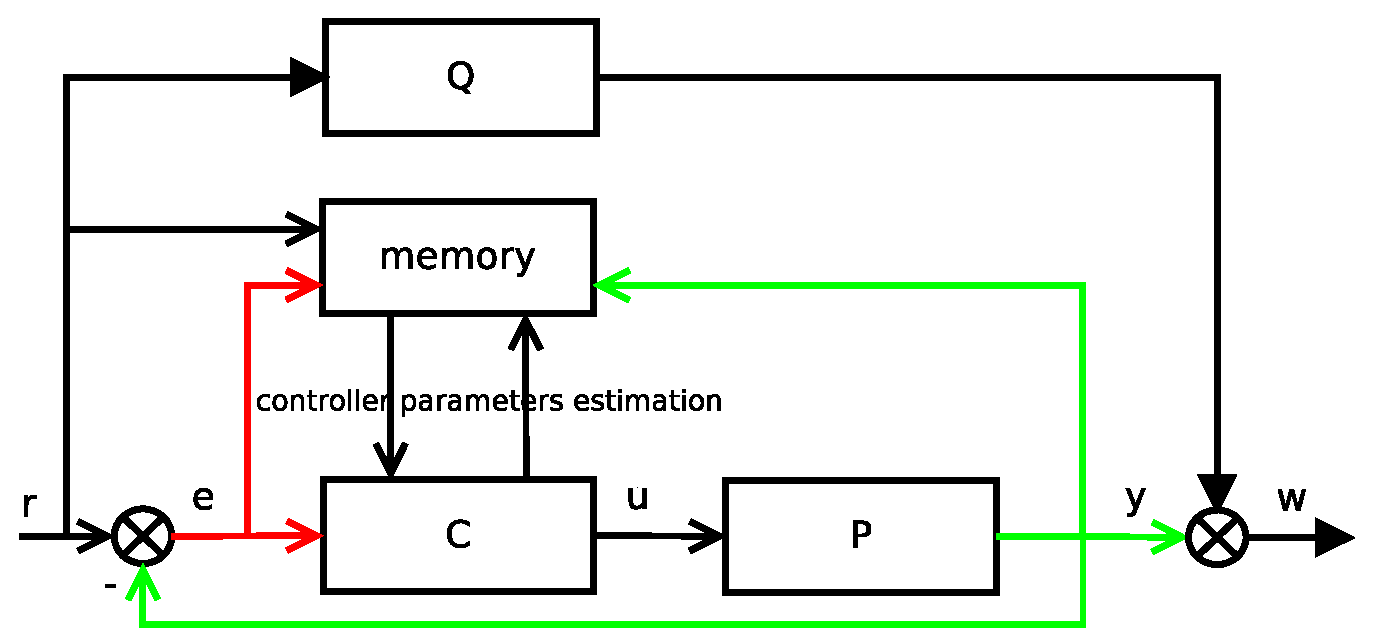
\includegraphics[scale=.22]{../diagrams/learning_system.eps}
  \label{fig:learning_system}
  \end{figure}

  \begin{figure}[!htb]
  \centering
  \includegraphics[scale=.2]{../pictures/function_f0.png}
  \end{figure}

\end{minipage}
\end{frame}

%-------------------------------------------------------------------------------------
\begin{frame}{\bf Adaptívne a učiace sa systémy}
\begin{minipage}{.5\textwidth}

  {\bf Adaptívny systém} \\
  PID regulátor

  \begin{equation} \label{eu_eqn}
  C(z) = \frac{b_{0} + b_{1}z^{-1} + b_{2}z^{-2}}{1 - z^{-1}} \nonumber
  \end{equation}

  \begin{figure}[!htb]
  %\centering
  \includegraphics[scale=.15]{../pid_ilc/pid_result.png}
  \end{figure}

\end{minipage}%
\begin{minipage}{.5\textwidth}

  {\bf Učiaci sa systém} \\
  Iterative learning controll

  \begin{equation} \label{eu_eqn}
  C(w) = \frac{\gamma}{1 - w^{-1}} \nonumber
  \end{equation}

  \begin{figure}[!htb]
  %\centering
  \includegraphics[scale=.15]{../pid_ilc/ilc_result_plant_error.png}
  \end{figure}

\end{minipage}
\end{frame}


%-------------------------------------------------------------------------------------
\begin{frame}{\bf Q-learning algoritmus}

Daná je množina stavov a akcií

\begin{align}
        s \in \mathbb{S} \nonumber\\
        a \in \mathbb{A} \nonumber
\end{align}

kde $\mathbb{S} \in \mathbb{R}^{N_s}$ a $\mathbb{A} \in \mathbb{R}^{N_a}$ .

Predpoklad : v prostedí existuje funkcia
\begin{align}
        s(n+1) = \lambda(s(n), a(n))
\end{align}

prechodová funkcia zo stavu $s(n)$ použitím akcie $a(n)$ - táto funkcia je ale agentovi neznáma.

Cieľom je nájsť takú postupnosť akcií $a \in \mathbb{A}$ pre ktorú bude maximálne

\begin{equation} \label{eu_eqn}
y = \prod_{i=1}Q_i(s_i, a_i)
\end{equation}



\end{frame}




%-------------------------------------------------------------------------------------
\begin{frame}{\bf Q-learning algoritmus - agent začlenený do prostredia}

\begin{figure}[!htb]
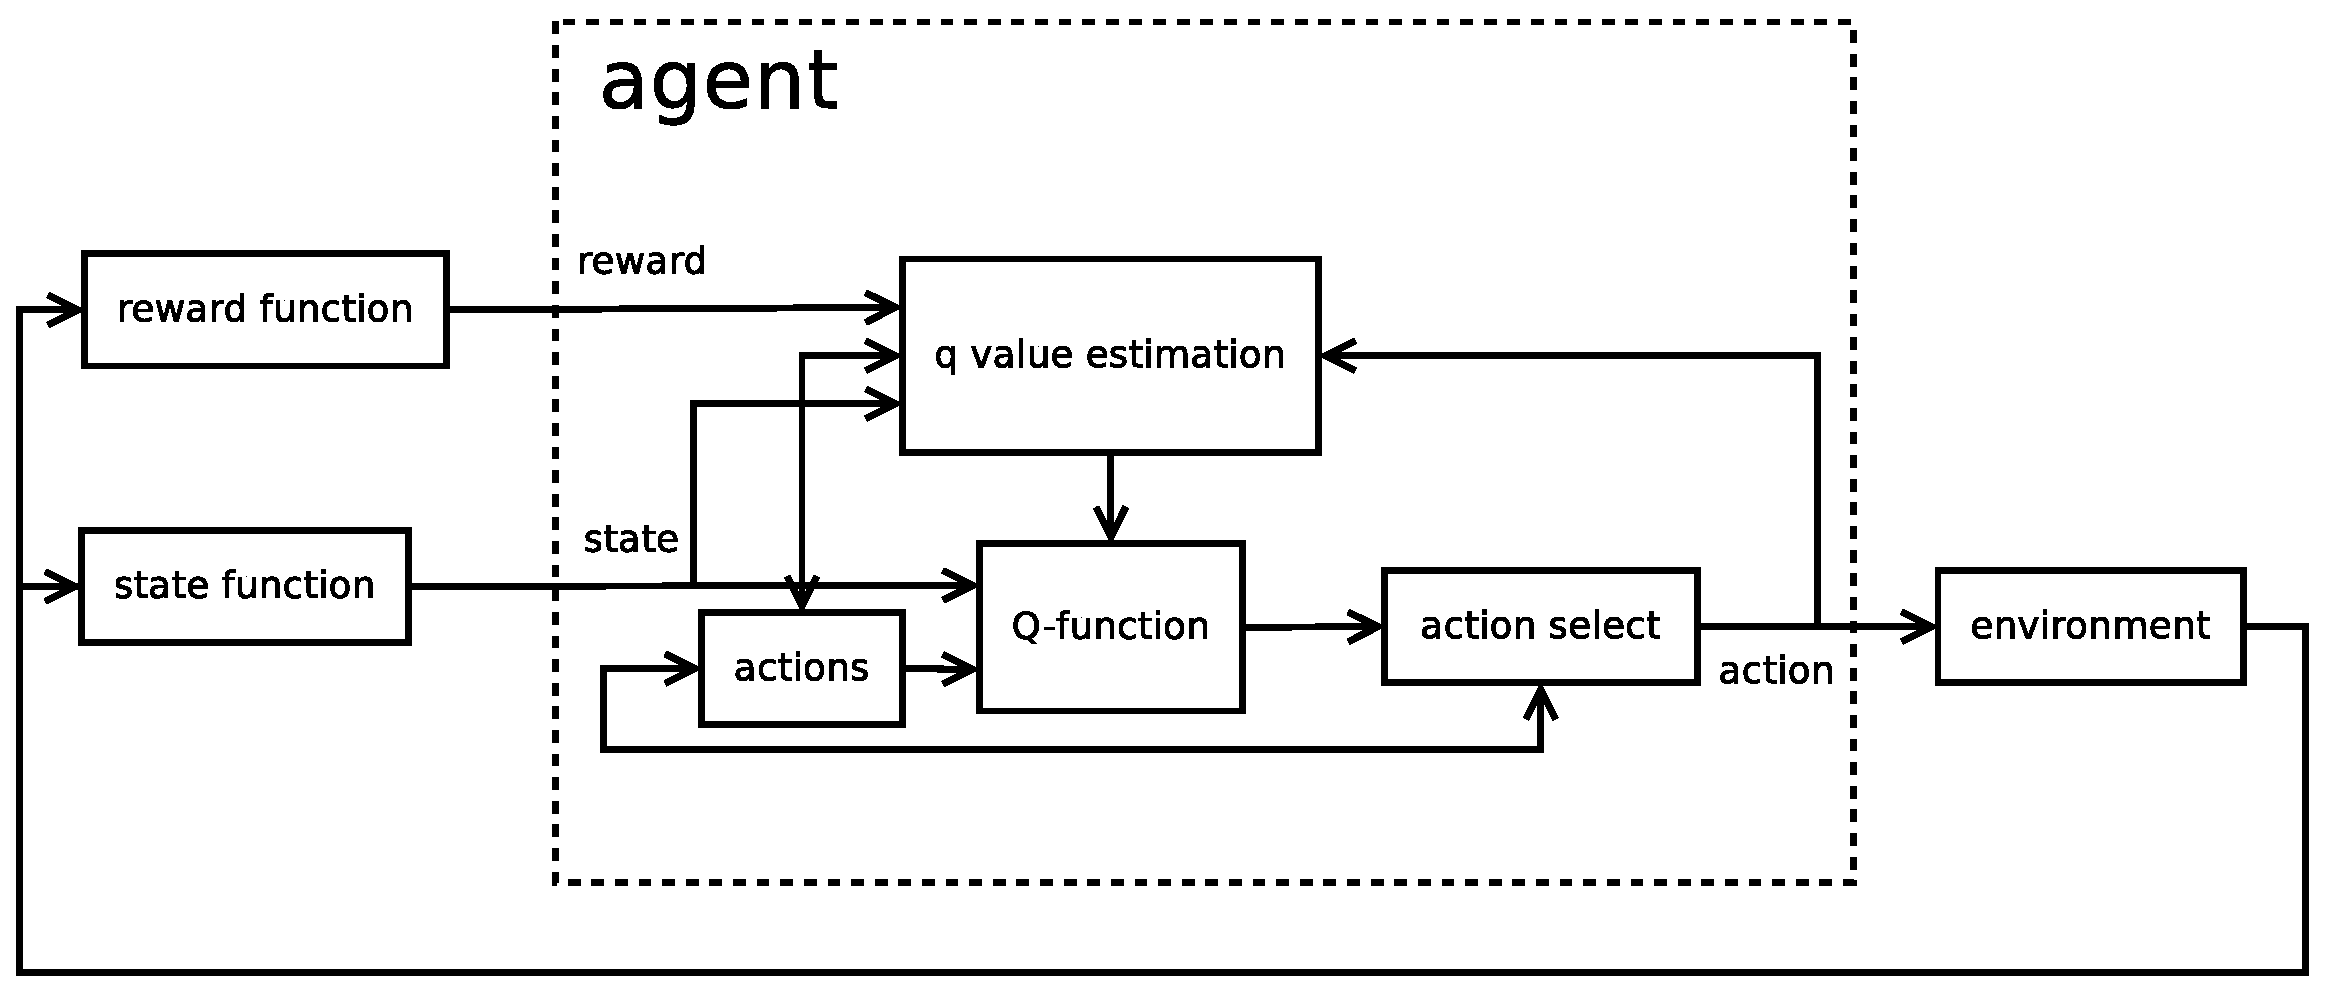
\includegraphics[scale=.3]{../diagrams/q_learning_agent.eps}
\end{figure}

\end{frame}




%-------------------------------------------------------------------------------------
\begin{frame}{\bf Q-learning algoritmus}

Daná je funkcia ohodnotení

\begin{equation} \label{eu_eqn}
Q(s,a) = R(s,a) + \gamma \max_{a' \in \mathbb{A}} Q'(s', a')
\end{equation}

kde \\
$R(s,a)$ je odmeňovacia funkcia, \\
$Q'(s',a')$ je odmeňovacia funkcia z ktorej sa agent dostal zo stavu "$s'$" \ vykonaním "$a$" \ do
stavu "$s$", \\
$\gamma$ je odmeňovacia konštanta a platí $\gamma \in (0, 1)$.

\end{frame}



%-------------------------------------------------------------------------------------
\begin{frame}{\bf Q-learning algoritmus}

\begin{figure}[!htb]
\includegraphics[scale=.5]{../diagrams/q_learning_table_01.eps}
\end{figure}

\end{frame}

%-------------------------------------------------------------------------------------
\begin{frame}{\bf Q-learning algoritmus}

\begin{figure}[!htb]
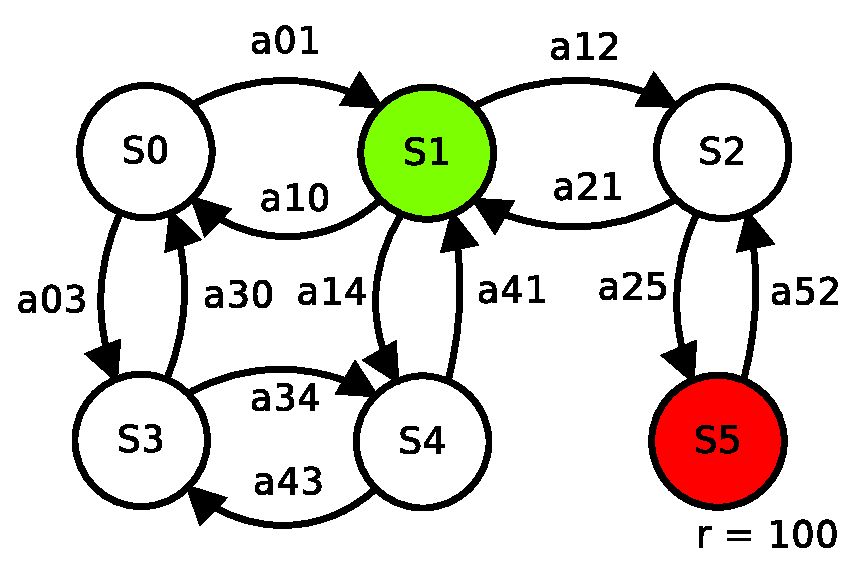
\includegraphics[scale=.5]{../diagrams/q_learning_table_02.eps}
\end{figure}

\end{frame}

%-------------------------------------------------------------------------------------
\begin{frame}{\bf Q-learning algoritmus}

\begin{figure}[!htb]
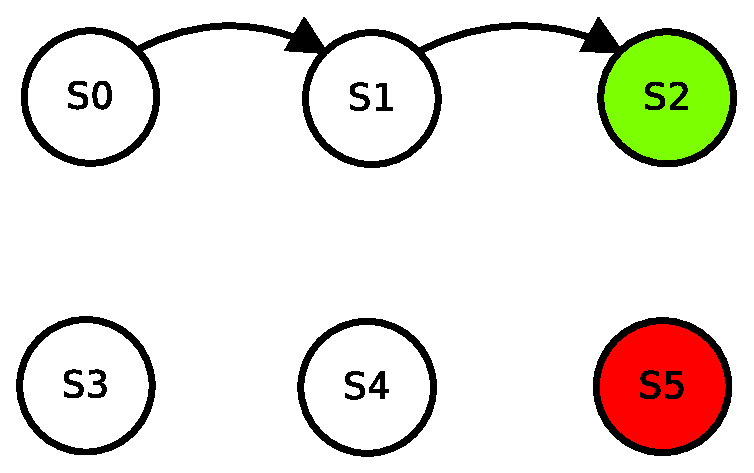
\includegraphics[scale=.5]{../diagrams/q_learning_table_03.eps}
\end{figure}

\end{frame}

%-------------------------------------------------------------------------------------
\begin{frame}{\bf Q-learning algoritmus}

\begin{figure}[!htb]
\includegraphics[scale=.5]{../diagrams/q_learning_table_04.eps}
\end{figure}

\end{frame}

%-------------------------------------------------------------------------------------
\begin{frame}{\bf Q-learning algoritmus}

\begin{figure}[!htb]
\includegraphics[scale=.5]{../diagrams/q_learning_table_05.eps}
\end{figure}

\end{frame}

%-------------------------------------------------------------------------------------
\begin{frame}{\bf Q-learning algoritmus}

\begin{figure}[!htb]
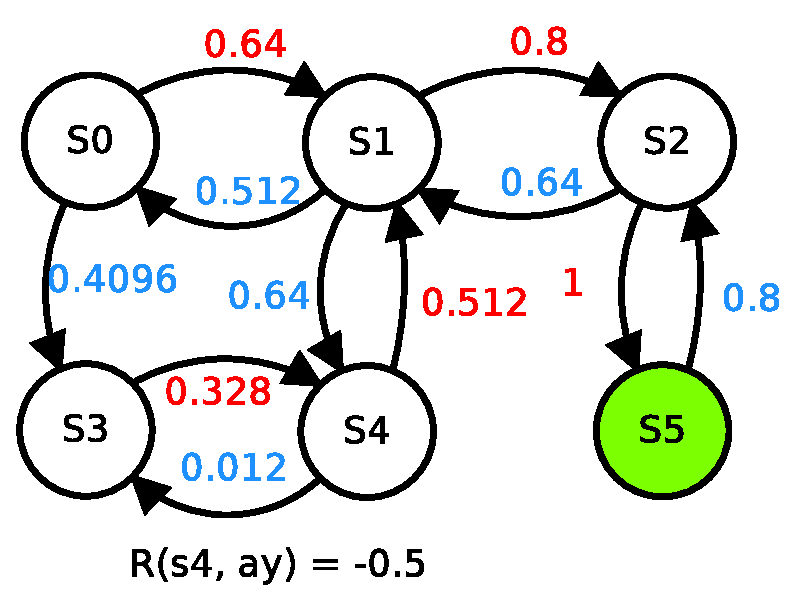
\includegraphics[scale=.5]{../diagrams/q_learning_table_06.eps}
\end{figure}

\end{frame}


%-------------------------------------------------------------------------------------
\begin{frame}{\bf Q-learning algoritmus}

Problémy tabuľkovej interpretácie $Q(s, a)$

\begin{itemize}
\item pre veľké ${N_s}\  alebo  {N_a}$\ narastajú pamäťové nároky
\item o nevyplnených $Q(s, a)$ vieme povedať nič
\item pre rozsiahle stavové priestory nevypočítateľné
\item ako aproximovať $Q(s, a)$?
\end{itemize}

\end{frame}


%-------------------------------------------------------------------------------------
\begin{frame}{\bf Q-learning algoritmus - aproximácia}

Neurónová sieť?
Utopická predstava :

\begin{figure}[!htb]
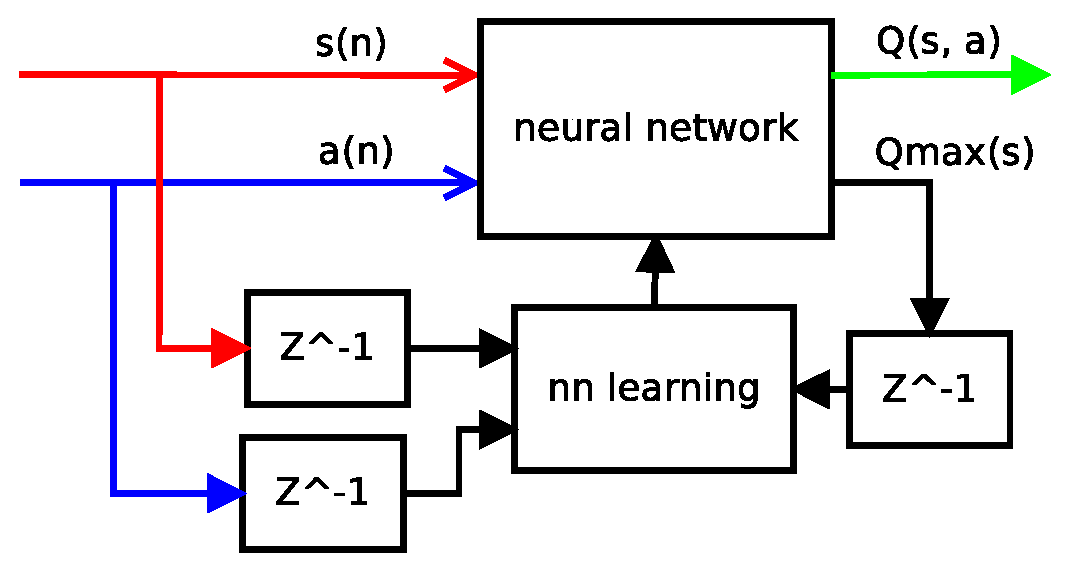
\includegraphics[scale=.5]{../diagrams/q_learning_nn.eps}
\end{figure}

prečo nedáva správne výsledky?
\end{frame}


%-------------------------------------------------------------------------------------
\begin{frame}{\bf Q-learning algoritmus - aproximácia}

\begin{figure}[!htb]
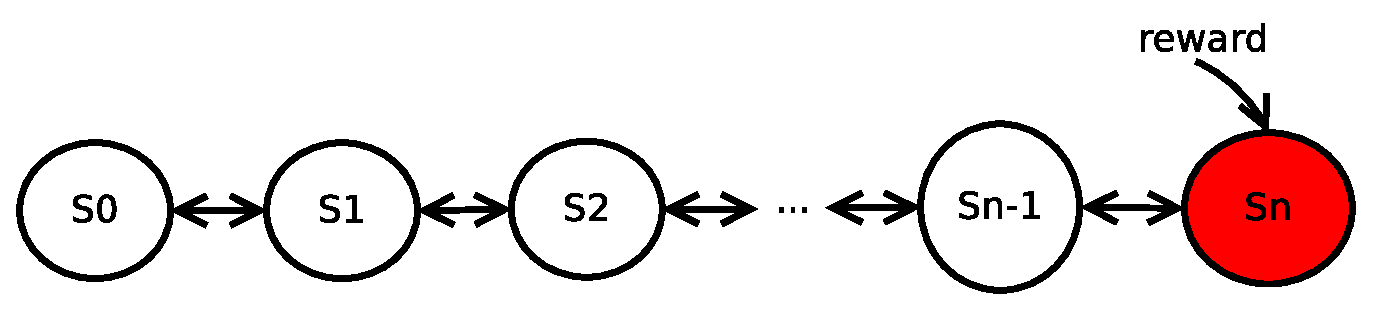
\includegraphics[scale=.5]{../diagrams/q_chain_problem.eps}
\end{figure}

Pre korektné vyplnenie hodnôt v $s_{n-1}$ sa vyžaduje korektá hodnota v $s_{n}$

\begin{align}
    Q(s_{0},a_{0}) &= R(s_{0},a_{0}) + \gamma \max_{a_{1}' \in \mathbb{A}} Q'(s_{1}, a'_{1}) \nonumber\\
    Q(s_{1},a_{1}) &= R(s_{1},a_{1}) + \gamma \max_{a_{2}' \in \mathbb{A}} Q'(s_{2}, a'_{2}) \nonumber\\
    Q(s_{2},a_{2}) &= R(s_{2},a_{2}) + \gamma \max_{a_{3}' \in \mathbb{A}} Q'(s_{3}, a'_{3}) \nonumber\\
    & \dots
\end{align}

\end{frame}



%-------------------------------------------------------------------------------------
\begin{frame}{\bf Q-learning algoritmus - aproximácia}

Učenie doprednej siete nie je homogénne! \\
- v priebehu učenia $Q(s,a)$ chaoticky osciluje okolo požadovanej hodnoty \\
- ani po 10-tkach milónoch iterácií sa hodnota neustáli na požadovanej hodnote


\end{frame}


%-------------------------------------------------------------------------------------
\begin{frame}{\bf Q-learning algoritmus - aproximácia}

Je možné zostaviť neurónovú sieť ktorá sa dá učiť lokálne?

\begin{figure}[!htb]
\includegraphics[scale=.35]{../pictures/gaussian.png}
\end{figure}

\end{frame}


%-------------------------------------------------------------------------------------
\begin{frame}{\bf Q-learning algoritmus - aproximácia}

Rozklad na bázické funkcie

\begin{align}
    f_j^a(\boldmath{X}) &= \sum\limits_{i=1}^{N_s}{ b_{1ji}(x_i - a_{1ji})^1 + b_{2ji}(x_i - a_{2ji})^2 + ...  }  \\
    f_j^a(\boldmath{X}) &= \sum\limits_{i=1}^{N_s}{max(0, b_{ji}(x_i - a_{ji}))}  \\
    f_j^b(\boldmath{X}) &= cos(\sum\limits_{i=1}^{N_s}{b_{ji}(x_i - a_{ji}) })  \\
    f_j^c(\boldmath{X}) &= e^{ \sum\limits_{i=1}^{N_s}{-b_{ji}\mid x_i - a_{ji} \mid} }  \\
    f_j^d(\boldmath{X}) &= e^{ \sum\limits_{i=1}^{N_s}{-b_{ji}(x_i - a_{ji})^2} }
\end{align}

\end{frame}


%-------------------------------------------------------------------------------------
\begin{frame}{\bf Q-learning algoritmus - aproximácia}

Ohliadnúc na charakter učiaceho algoritmu

\begin{equation} \label{eu_eqn}
Q(s,a) = R(s,a) + \gamma \max_{a' \in \mathbb{A}} Q'(s', a') \nonumber
\end{equation}



\begin{minipage}{.5\textwidth}
  boli zvolené bázické funkcie

  \begin{align}
      f_j^c(\boldmath{X}) &= e^{ \sum\limits_{i=1}^{N_s}{-b_{ji}\mid x_i - a_{ji} \mid}} \nonumber \\
      f_j^d(\boldmath{X}) &= e^{ \sum\limits_{i=1}^{N_s}{-b_{ji}(x_i - a_{ji})^2} } \nonumber
  \end{align}

kde

  \begin{align}
      \mid x \mid = \lim_{\epsilon \to 0} \sqrt[2]{x^2 + \epsilon}  \nonumber
  \end{align}


\end{minipage}%
\begin{minipage}{.5\textwidth}

  \begin{figure}[!htb]
  %\centering
  \includegraphics[scale=.2]{../pictures/gaussian_1D.png}
  \end{figure}

\end{minipage}





\end{frame}



%-------------------------------------------------------------------------------------
\begin{frame}{\bf Q-learning algoritmus - aproximácia}

Rozklad na bázické funkcie

\begin{align}
    f_j(\boldmath{X}) = e^{ \sum\limits_{i=1}^{N_s}{-b_{ji}(x_i - a_{ji})^2} }
\end{align}

pre symetrické prechody medzi stavmi možno zjednodušiť na

\begin{align}
    f_j(\boldmath{X}) = e^{ -b_j\sum\limits_{i=1}^{N_s}{(x_i - a_{ji})^2} }
\end{align}

A ich kombinácia

\begin{align}
    y(\boldmath{X})&= \sum\limits_{j=1}^{N}w_jf_j(\boldmath{X}) \nonumber \\
                  &+ \sum\limits_{j=1}^{N}{\sum\limits_{i=1}^{j}v_{ji}f_j(\boldmath{X})f_i(\boldmath{X})}
\end{align}


\end{frame}







%-------------------------------------------------------------------------------------
\begin{frame}{\bf Q-learning algoritmus - aproximácia}

Stavenie parametrov :

\begin{itemize}
\item bázicke funkcie musia rovnomerne pokryť stavový priestor
\item parameter $a_{ji}$ reprezentuje posunutie Gaussovej krivky - bod s najväčou funkčnou hodnotou.
\item parameter $b_{j}$ reprezentuje strmosť krivky
\end{itemize}

\end{frame}

%-------------------------------------------------------------------------------------
\begin{frame}{\bf Q-learning algoritmus - aproximácia}

Paramatre $a_{ji}$ - pokrytie stavového priestoru do oblastí podľa veľkosti $R(s, a)$
Využije sa princíp Kohonenovej siete - najbližšie vzory $a_j$ sa posunú podľa vstupných
vektorov tak aby vrchol Gaussovej krivky ležal v ťazisku.
\\
\begin{itemize}
\item na začiatku sa zvolia $a_{ji}$ náhodne
\item spočítajú sa vzdialenosti od predloženého vstupu $d_j = \mid X - a_{j} \mid$
\item nájde sa také $k$ kde  $\forall{j} : d_k \leq d_j$
\item spočíta sa krok učenia $\eta' = \eta_1 \mid y_r \mid$
\item upravia sa parametre $a_{ki} = (1 - \eta')a_{ki} + \eta' x_{i}$
\end{itemize}

kde \\
$X$ je vstupný vektor \\
$y_r$ je požadovaný výstup \\
$\eta_1$ je krok učenia \\

\end{frame}

%-------------------------------------------------------------------------------------
\begin{frame}{\bf Q-learning algoritmus - aproximácia}

Paramatre $b_{j}$ - určuje strmosť krivky

\begin{itemize}
\item stanoví sa chyba $e(n) = y_r(n) - y(n)$
\item pre každú bázickú funkciu  $b_j(n+1)= b_j(n) -\eta_2 e(n)w_j(n)$
\item skontroluje sa $b_j \in (0, -\infty)$
\end{itemize}

kde \\
$y_r$ je požadovaný výstup \\
$y$ je výstup\\
$\eta_2$ je krok učenia \\

\end{frame}


%-------------------------------------------------------------------------------------
\begin{frame}{\bf Q-learning algoritmus - aproximácia}

Paramatre $w_{j}$ - váhové parametre

\begin{itemize}
\item stanoví sa chyba $e(n) = y_r(n) - y(n)$
\item pre každé $w_{j}$ : $w_j(n+1)= w_j(n) -\eta_3 e(n)y_j(n)$
\item skontroluje sa $w_j \in (-a, a)$
\end{itemize}

kde \\
$\eta_3$ je krok učenia \\
$a$ je maximálny rozsah váh \\
\end{frame}


%-------------------------------------------------------------------------------------
\begin{frame}{\bf Výsledky experimentov - schéma priebehu experimentov}

\begin{figure}[!htb]
\centering
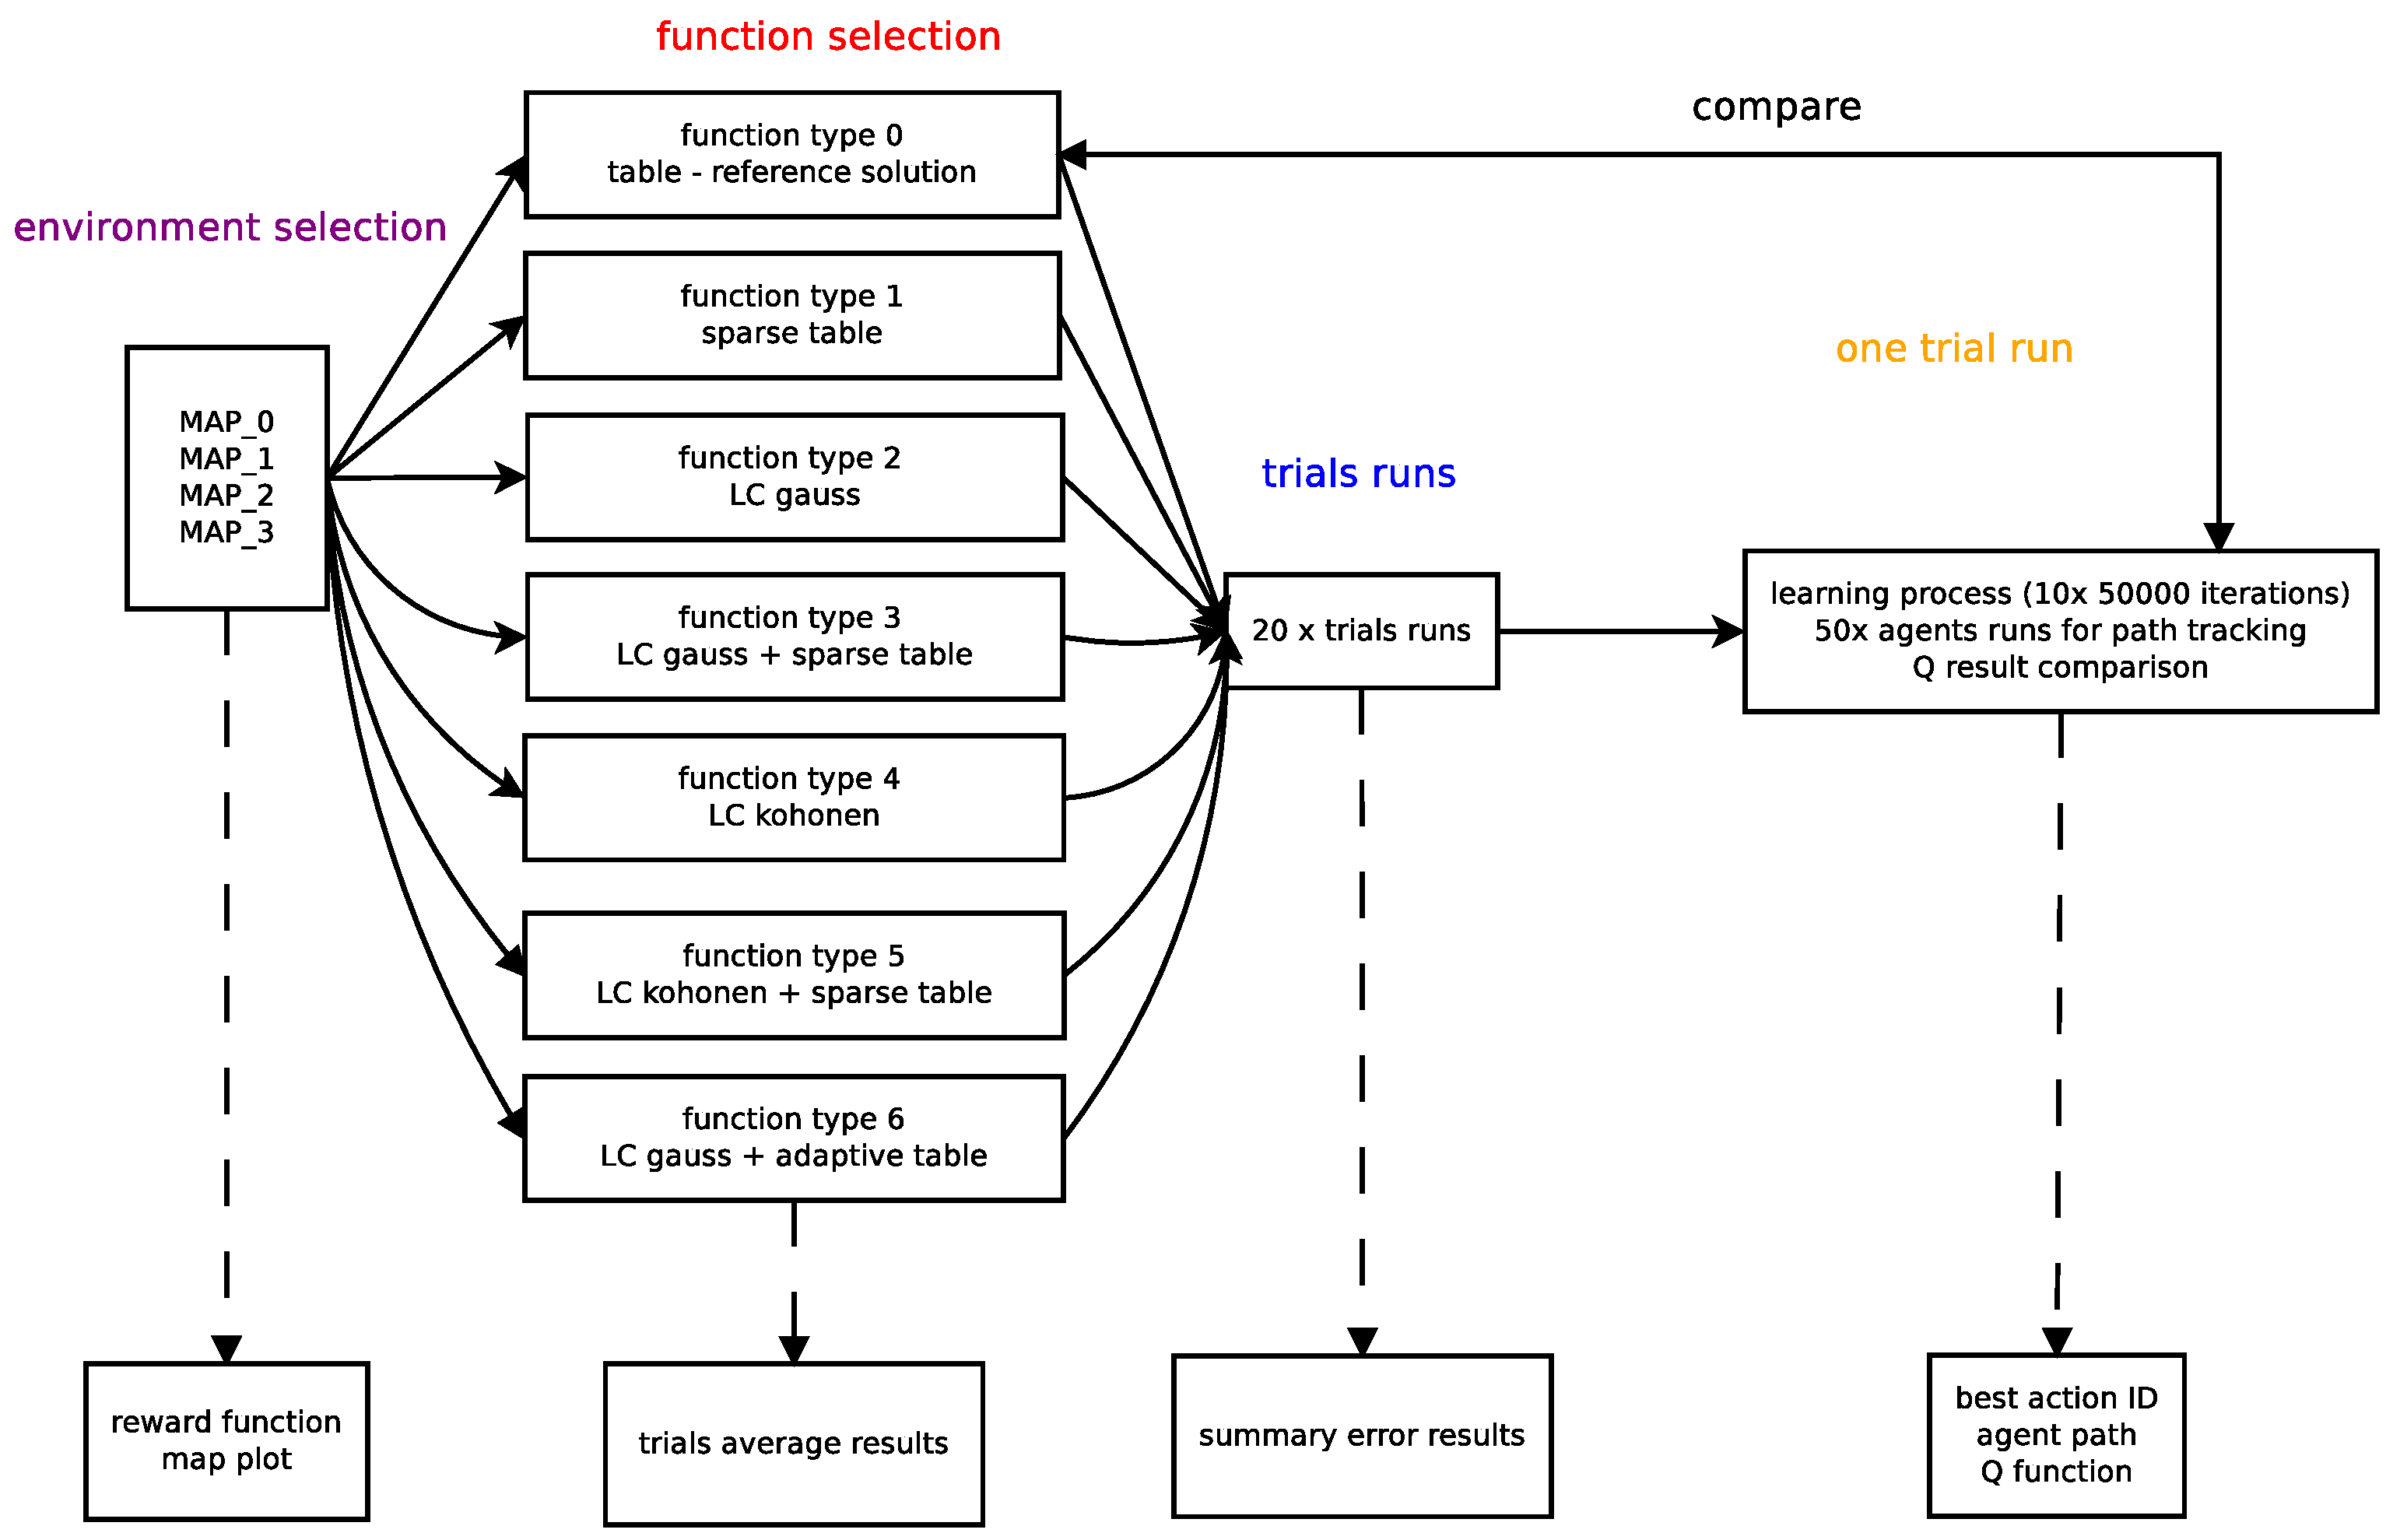
\includegraphics[scale=.22]{../diagrams/experiment_map_q_learning.eps}
\end{figure}

\end{frame}


%-------------------------------------------------------------------------------------
\begin{frame}{\bf Výsledky experimentov - bloková schéma}

\begin{figure}[!htb]
\centering
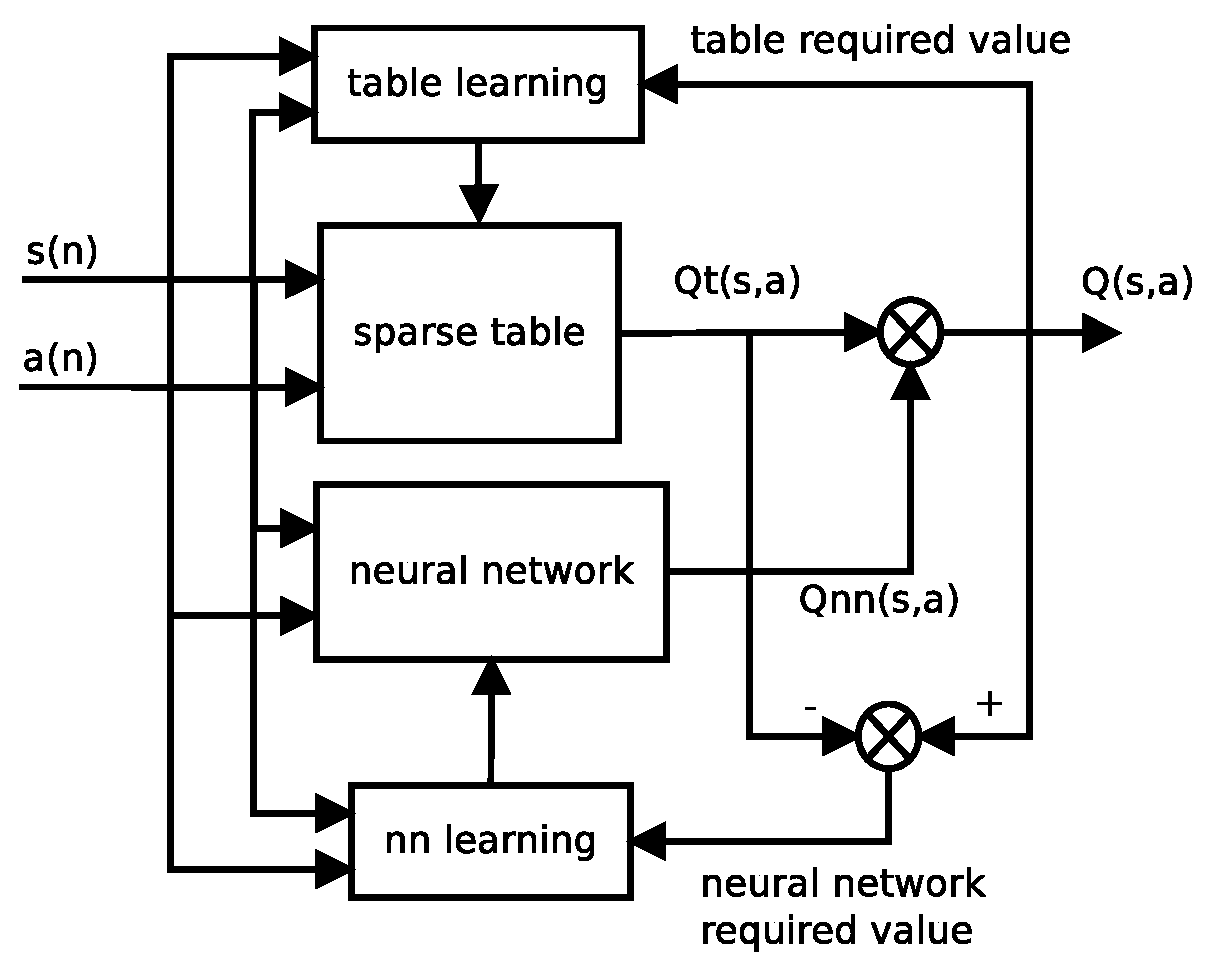
\includegraphics[scale=.4]{../diagrams/q_learning_hybrid.eps}
\end{figure}

\end{frame}


%-------------------------------------------------------------------------------------
\begin{frame}{\bf Výsledky experimentov - podmienky}

\begin{itemize}
\item 50000 iterácií učenia
\item Q-learning
\begin{equation} \label{eu_eqn}
Q(s,a) = \alpha(Q'(s,a)) + (1 - \alpha)(R(s,a) + \gamma \max_{a' \in \mathbb{A}} Q'(s', a')) \nonumber
\end{equation}

\item $R(s, a) =$ náhodná mapa s 1 cieľovým stavom
\item hodnoty $R(s, a) \in \langle -1, 1 \rangle$
\item $\gamma = 0.98$ a $\alpha = 0.7$

\item hustota referenčného riešenia = 1/32  (4096 stavov)
\item počet akcií v každom stave = 8
\item hustota riedkej tabuľky = 1/8  (1:16 pomer)
\item počet bázických funkcií = 64
\item rozsah parametrov
    \begin{itemize}
      \item a\_range = 1.0
      \item b\_range = 200.0
      \item w\_range = 10.0
    \end{itemize}
\end{itemize}

\end{frame}


%-------------------------------------------------------------------------------------
\begin{frame}{\bf Výsledky experimentov - funkcia R(s), mapa 1}

\begin{figure}[!htb]
\centering
\includegraphics[scale=.4]{../../results_q_learning/map_1/reward_value_surface.png}
\end{figure}

\end{frame}



%-------------------------------------------------------------------------------------
\begin{frame}{\bf Výsledky experimentov - mapa najlepších akcií}

\begin{minipage}{.5\textwidth}

\begin{figure}[!htb]
\centering
\includegraphics[scale=.2]{../../results_q_learning/map_1/function_type_1/iterations_10/action_best_value_log_surface.png}
\caption{sparse table}
\end{figure}

\end{minipage}%
\begin{minipage}{.5\textwidth}

\begin{figure}[!htb]
\centering
\includegraphics[scale=.2]{../../results_q_learning/map_1/function_type_2/iterations_10/action_best_value_log_surface.png}
\caption{linear combination Gauss}
\end{figure}


\end{minipage}
\end{frame}


%-------------------------------------------------------------------------------------
\begin{frame}{\bf Výsledky experimentov - mapa najlepších akcií}

\begin{minipage}{.5\textwidth}

\begin{figure}[!htb]
\centering
\includegraphics[scale=.2]{../../results_q_learning/map_1/function_type_3/iterations_10/action_best_value_log_surface.png}
\caption{sparse table + linear combination Gauss}
\end{figure}


\end{minipage}%
\begin{minipage}{.5\textwidth}

\begin{figure}[!htb]
\centering
\includegraphics[scale=.2]{../../results_q_learning/map_1/function_type_4/iterations_10/action_best_value_log_surface.png}
\caption{sparse table + linear combination + multiplication Gauss}
\end{figure}


\end{minipage}
\end{frame}










%-------------------------------------------------------------------------------------
\begin{frame}{\bf Výsledky experimentov - chybové funkcie}

\begin{minipage}{.5\textwidth}

\begin{figure}[!htb]
\centering
\includegraphics[scale=.2]{../../results_q_learning/map_1/function_type_1/q_learning_error.png}
\caption{sparse table}
\end{figure}

\end{minipage}%
\begin{minipage}{.5\textwidth}

\begin{figure}[!htb]
\centering
\includegraphics[scale=.2]{../../results_q_learning/map_1/function_type_2/q_learning_error.png}
\caption{linear combination Gauss}
\end{figure}


\end{minipage}
\end{frame}


%-------------------------------------------------------------------------------------
\begin{frame}{\bf Výsledky experimentov - chybové funkcie}

\begin{minipage}{.5\textwidth}

\begin{figure}[!htb]
\centering
\includegraphics[scale=.2]{../../results_q_learning/map_1/function_type_3/q_learning_error.png}
\caption{sparse table + linear combination Gauss}
\end{figure}


\end{minipage}%
\begin{minipage}{.5\textwidth}

\begin{figure}[!htb]
\centering
\includegraphics[scale=.2]{../../results_q_learning/map_1/function_type_4/q_learning_error.png}
\caption{sparse table + linear combination + multiplication Gauss}
\end{figure}


\end{minipage}
\end{frame}





%-------------------------------------------------------------------------------------
\begin{frame}{\bf Výsledky experimentov - max Q(s, a)}

\begin{minipage}{.5\textwidth}

\begin{figure}[!htb]
\centering
\includegraphics[scale=.2]{../../results_q_learning/map_1/function_type_0/iterations_10/q_learning_result.png}
\caption{reference table}
\end{figure}

\end{minipage}%
\begin{minipage}{.5\textwidth}

\begin{figure}[!htb]
\centering
\includegraphics[scale=.2]{../../results_q_learning/map_1/function_type_3/iterations_10/q_learning_result.png}
\caption{sparse table + linear combination Gauss}
\end{figure}


\end{minipage}
\end{frame}



%-------------------------------------------------------------------------------------
\begin{frame}{\bf Výsledky experimentov - trials progress}

\begin{figure}[!htb]
\centering
\includegraphics[scale=.36]{../../results_q_learning/map_1/trials_average_results_progress.png}
\end{figure}

\end{frame}



%-------------------------------------------------------------------------------------
\begin{frame}{\bf Výsledky experimentov - trials average}

\begin{figure}[!htb]
\centering
\includegraphics[scale=.36]{../../results_q_learning/map_1/trials_average_results.png}
\end{figure}

\end{frame}


%-------------------------------------------------------------------------------------
\begin{frame}{\bf Ďakujem za pozornosť}

\begin{figure}[!htb]
\centering
\includegraphics[scale=.15]{../pictures/me.jpg}
\end{figure}

\centerline{michal.chovanec@yandex.ru}

\end{frame}

\end{document}
